\begin{figure}[t]
    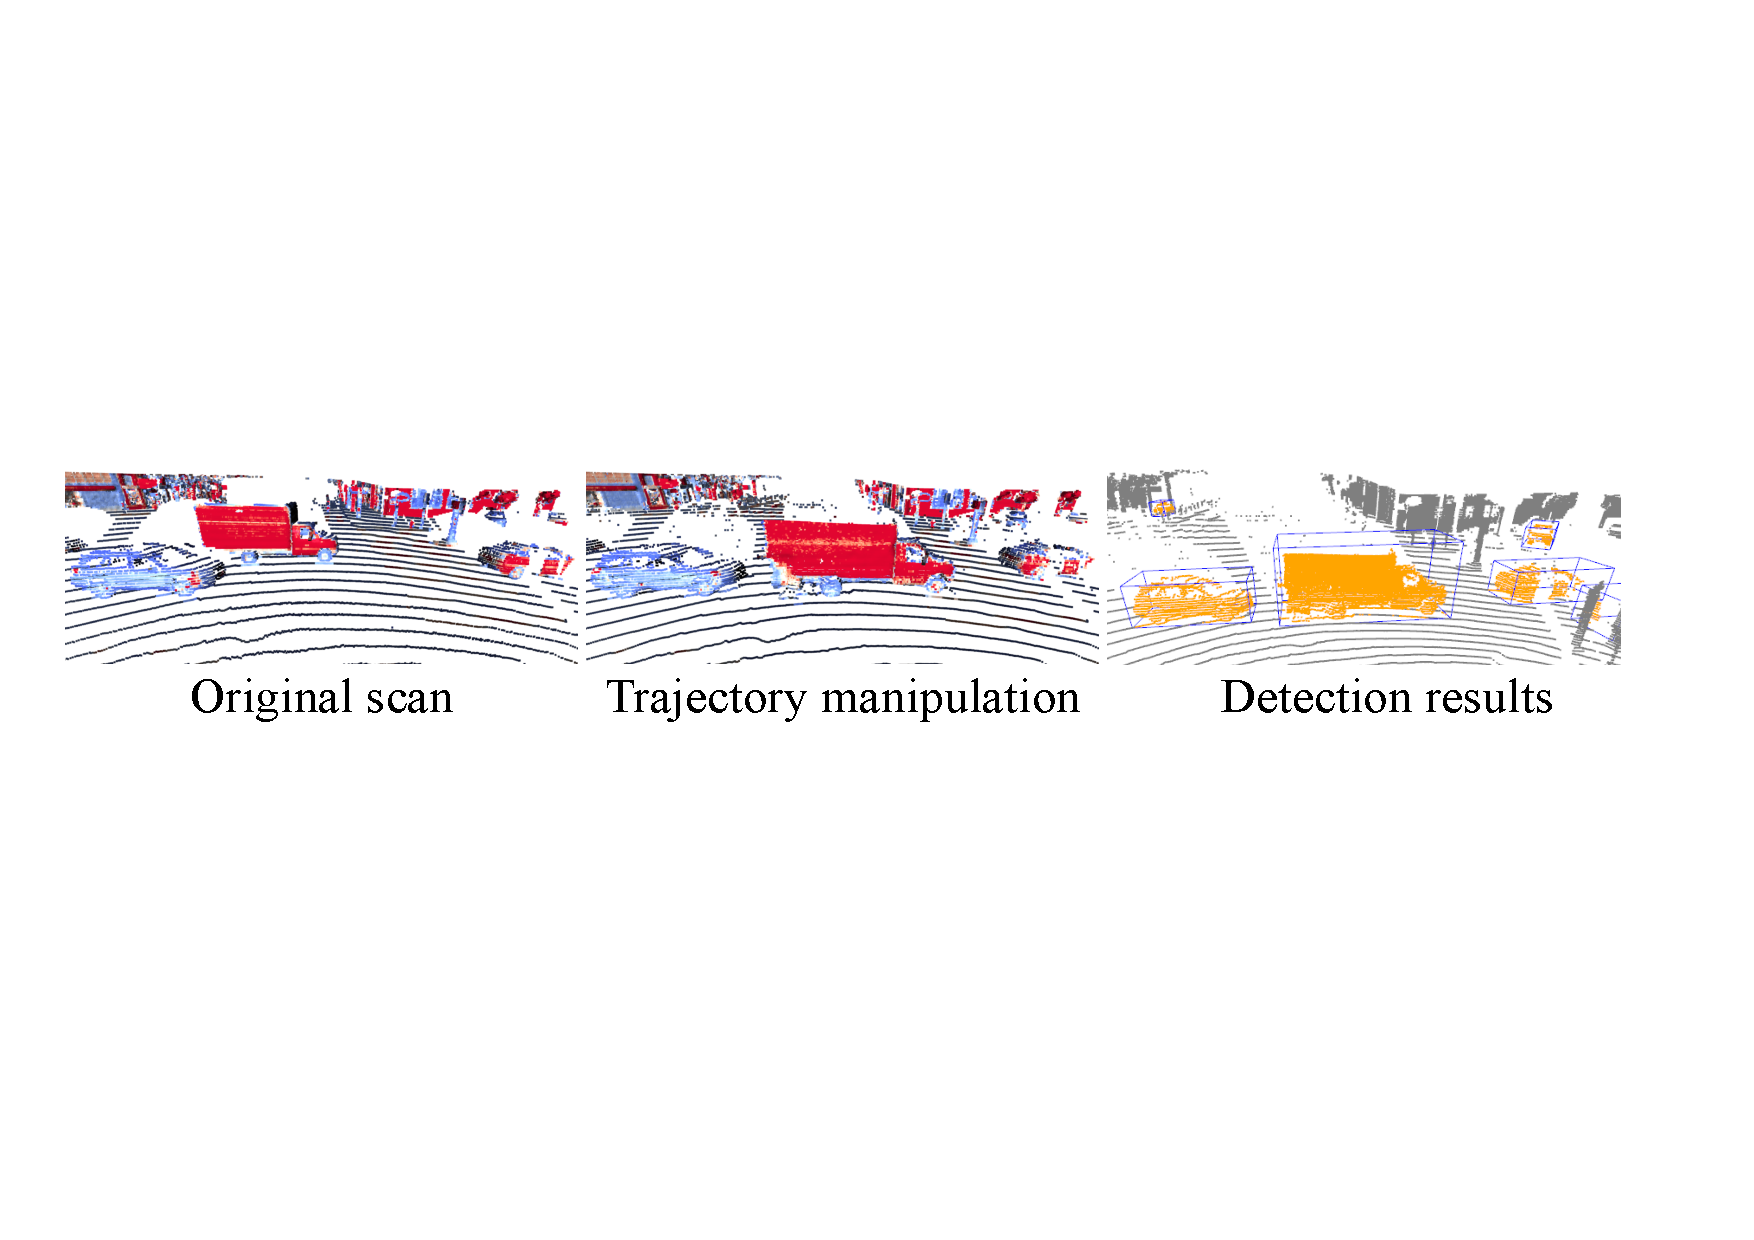
\includegraphics[width=1.0\columnwidth]{Figures/trajectory_manipulation.pdf}
    
    \caption{Qualitative results of object trajectory manipulation. The truck can be successfully detected after manipulation, indicating high-realism LiDAR re-simulation achieved by \dynfl.}
    % \caption{The middle figure showcase the trajectory manipulation application on the moving truck. The images are color-coded by the intensity values (0 \bwrDyNFL~0.25). The object detection results on the LiDAR scan after manipulation is shown on the right, we annotate the points in \textcolor{orange}{orange} if they are within the detection bounding boxes.}
    \label{fig:traj}
    
\end{figure}